%Resume penggunaan aplikasi testing webservice
%judul jurnal hari ke 1  IMPLEMENTASI REST WEB SERVICE UNTUK SALES ORDER DAN SALES TRACKING BERBASIS MOBILE
%judul jurnal hari ke 2  Penerapan Teknologi Web Service Untuk Integrasi Layanan Puskesmas dan Rumah Sakit
%judul jurnal hari ke 3  PEMANFAATAN GOOGLE MAPS API UNTUK PEMBANGUNAN SISTEM INFORMASI MANAJEMEN BANTUAN LOGISTIK PASCA BENCANA ALAM BERBASIS MOBILE WEB( Studi Kasus : Badan Penanggulangan Bencana Daerah Kota Yogyakarta ) 
%judul jurnal hari ke 4 WEB SERVICE SEBAGAI SOLUSI INTEGRASI DATA PADA SISTEM INFORMASI AKADEMIK UNIVERSITAS BINA DARMA

%Kelompok 5 D4 TI - 2B
%Fransiscus Ivan Martongam      1164039 
%Lalita Chandiany Adiputri      1164043
%Eko Cahyono Putro              1164035
%Lidwina Triniska Gulo          1164044
%Sulpadianti Bunyamin           1164096


\section{Pengenalan WebService}
Web Services dengan arsitektur REST digunakan oleh berbagai macam jenis client seperti mobile, Web, dan Desktop.
Dapat membantu perusahaan untuk melakukan pelacakan, tracking terhadap tenaga penjual yang ditugaskan untuk menawarkan 
barang atau penagihan ke pelanggan. Dengan REST Web Services yang akan dibuat perusahaan akan dapat memastikan
bahwa semua tenaga penjual akan mengunjungi pelanggan sesuai dengan target yang sudah ditentukan oleh perusahaan.


\section{Arsitektur Web Services}
Architektur Web Service memiliki tiga komponen utama diantaranya yaitu Service provider adalah Penyedia web service yang berfungsi
menyediakan kumpulan web services yang dapat diaksesoleh pengguna.Service requesto adalah aplikasi yang bertindak sebagai pengguna yang
melakukan permintaan layanan (berupaweb services) keservice provider.Service registry adalah tempat dimana service provider 
mempublikasikan layanannya. Pada arsitekturWeb service,Service registry bersifat opsional.

\ref{arsitektur}
\centerline{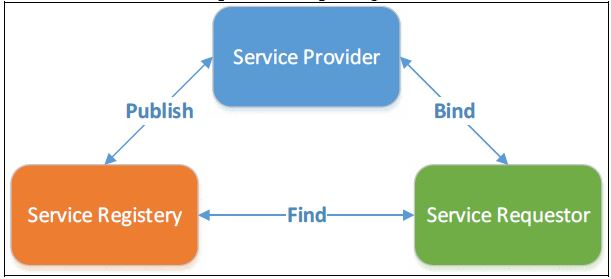
\includegraphics[width=1\textwidth]{figures/arsitektur.PNG}}
\caption{arsitektur web service}
\lable{arsitektur}
\end{figure}


\section{rest dalam penggunaan testing web service}
REST adalah filosofi desain yang mendorong untuk menggunakan protokol dan fitur yang sudah ada pada Web. Pada web services akan dapat memaksimalkan kinerja web services terutama pada performa, skalabilitas, dan kemudahan untuk dimodifikasi. Bentuk web service menggunakan REST style digunakan sebagai backend dari aplikasi berbasis mobile karena cara aksesnya  mudah dan hasil data yang dikirimkan berformat JSON sehingga ukuran file menjadi lebih kecil. 


\section{web api}
Web API adalah antar muka program dari sistem yang dapat diakses lewat method dan
header pada protokol HTTP yang standar. Web API dapat diakses dari berbagai macam HTTP
client seperti browser dan perangkat mobile. Web API juga memiliki keuntungan karena
menggunakan infrastruktur yang juga digunakan oleh web terutama untuk penggunaan caching
dan concurrency.


\section{Perancangan Sistem}
Aplikasi yang akan dibuat terdiri dari dua bagian besar yaitu aplikasi yang ada pada bagian client dan bagian server. 
Aplikasi yang ada di server bertugas menyediakan data yang dapat digunakan oleh aplikasi client, aplikasi client digunakan
untuk meminta data dari aplikasi yang ada di server.Web services dipilih dengan beberapa pertimbangan yaitu agar 
memudahkanpembangunan proses bisnis yang dapat digunakan untuk berbagai macam client tanpa harus membuat proses 
tersebut secara spesifik berdasarkan teknologi client yang digunakan.


\section{Implementasi Web service Berbasis ASP.NET}
Dalam proses pembuatan Web Services berbasis ASP.NET terdapat beberapa services atau fungsi-fungsi
yang dibuat untuk mengakses database SQL Server. Services-services tersebut yang nantinya dipanggil 
dan digunakan untuk membangun sistem integrasi layanan puskesmasdan rumah sakit berbasis Web Services.
Proses integrasi sistem dengan Web Services berbasis asp dapat dilakukan dengan penggunaan dokumen WSDL
yang dapat diakses pada alamat WSDL-nya http://192.168.1.100:8080/wsrs/Service.asmx?WSDL dan hasil dari skema WSDLnya.


\section{Implementasi Web service Berbasis PHP}
Pembuatan Web Services berbasis PHP dan database MySQL, terdapat  services atau fungsi yang sama 
dengan Web Services yang dibuat dengan ASP.NET. Sevices tersebut akan dipanggil dan digunakan untuk 
integrasi kedalam system berbasis Web Services. Beberapa fungsi yang terbentuk adalah sama dengan fungsi 
yang terbentuk pada hasil pembuatan Web Services berbasis ASP NET.


\section{Hasil Integrasi Web Services}
Sistem integrasi  layanan yang terdapat pada rumah sakit yang dimaksudkan menggunakan teknologi Web Services 
yang berbeda dan database yang berbeda pula. Rumah sakit AMC menggunakan database MySQL, dan PHP sebagai Web Servicesnya.
Kemudian untuk Rumah sakit umum menggunakan SQL Server sebagai databasenya, dan ASP.NET sebagai tool untuk membuat Web Servicesnya.


\section{Hasil Sistem integrasi  layanan puskesmas dan rumah sakit}
Layanan informasi merupakan halaman awal yang ditampilkan ketika client tersebut diakses menggunakan web browser. 
Setelah Itu pengguna melakukan pemilihan kriteria kelengkapan rumah sakit, pengguna harus mengisi data-data pasien yang mendaftar pada rumah sakit. Selanjutnya user  menampilkan data dokter, data kamar, data fasilitas, data pasien, dan juga data registrasi pasien pada rumah sakit.


\section{Analisis Hasil Pengujian dan Implementasi}
Aplikasi berjalan sesuai dengan analisis masalah dan kebutuhan sistem.
Pengujian sistem yang pertama dilakukan adalah testing pada web service itu sendiri 
dan dilanjutkan dengan testing pada fungsi-fungsi  yang terdapat pada masing-masing web service. 
selanjutnya dilakukan testing aplikasi web service melalui aplikasi web interface yang menggunakan bahasa pemrograman ASP.NET dan PHP.
Web Service yang berfungsi sebagai Middleware serta melakukan pertukaran data dalam format XML melalui sebuah jaringan dengan menggunakan protokol standar internet.


\section {Google Map Service}
Google Map Service adalah sebuah jasa peta global virtual gratis dan online yang
disediakan oleh perusahaan Google. Google Maps dapat ditemukan di alamat
http://maps.google.com.Google Maps menawarkan peta yang dapat diseret dan gambar
satelit untuk seluruh dunia.Google Maps juga menawarkan pencarian suatu tempat dan
rute perjalanan.
\subsection {Google Maps API }
Google Maps API adalah sebuah layanan (service) yang diberikan oleh Google
kepada para pengguna untuk memanfaatkan Google Map dalam mengembangkan
aplikasi. Google Maps API menyediakan beberapa fitur untuk memanipulasi peta, dan
menambah konten melalui berbagai jenis services yang dimiliki, serta mengijinkan
kepada pengguna untuk membangun aplikasi enterprise di dalam websitenya.


\section{Global Positioning System (GPS)}
Global Positioning System, adalah sistem atau sarana yang digunakan untuk memberikan informasi dimana keberadaan pengguna secara umum dipermukaan bumi yang berbasiskan satelit. Data dikirim dengan data digital. GPS dapat digunakan dimanapun juga dalam 24 jam. Posisi unit GPS akan ditentukan berdasarkan titik-titik koordinat latitude dan longitude, maka GPS bisa membantu menunjukan arah. 


\section{Geolocation}
Geolocation adalah sebuah cara untuk mengetahui suatu lokasi di dunia. Ada beberapa metode untuk menemukan lokasi, yaitu dengan IP address, sambungan wireless atau BTS, dan dedicated GPS atau embeded GPS pada telepon seluler. Geolocation selain menggunakan data koordinat latitude, selain itu geolocation juga menggunakan longitude yang dimiliki oleh komputer atau telepon seluler.


\section{Framework CodeIgniter}
CodeIgniter merupakan salah satu dari sekian banyak framework PHP yang  bertujuan dari pembuatan framework CodeIgniter ini adalah untuk menghasilkan framework  yang dapat digunakan untuk pembuatan proyek website secara lebih cepat dibandingkan dengan pembuatan website secara manual.
Salah satu keuntungan menggunakan framework codeigniter adalah, gratis, berjalan di php versi 4 dan 5, ringan dan cepat, mempunyai fitur-fitur yang lengkap dan menggunakan metode MVC (Model View Controller).



\section{Project Management and requirement}
Data warehouse yang dikembangkan adalah data warehouse yang dioptimasi untuk kepentingan evaluasi akademik Fakultas Teknologi Informasi. Fungsi evaluasi mencakup nilai mahasiswa, absensi dan hasil studi yang dapat dianalisa berdasarkan program studi, tahun ajaran, lokasi kuliah, dan angkatan mahasiswa. Berdasarkan pengumpulan data yang dilakukan, dilakukan analisa kebutuhan yaitu: Model data warehouse yang mampu digunakan oleh EIS, Dibutuhkan sebuah metode distribusi yang bersifat independen, sumber data yang mampu menampilkan laporan dan analisa


\section{Permodelan Data Warehouse Dimensional}
Sebagai sumber data untuk data warehouse, digunakan sumber data operasional yang menyimpan data harian dari sistem akademik. Database harian yang digunakan  oracle DBMS 6 yang menyimpan data–data akademik yaitu: mahasiswa, rencana studi, nilai, absensi, mata kuliah, jadwal, kurikulum, pembimbing akademik, dan lainnya. Untuk model skema yang digunakan star schema, dimana satu tabel fakta dikelilingi oleh beberapa tabel dimensi. 


\section{Pengembangan Model Distribusi Web Service}
Model distribusi data warehouse yang akan dikembangkan berbasis web service dengan framework WSF/PHP.    
Web service pada penelitian ini dapat diakses menggunakan SOAP (Simple Object Access Protocol) dengan transport layer http. 
Tiap client yang mengakses harus membuat instance dari kelas WSClient dan mengirim XML format request. 
Untuk dapat digunakan aplikasi desktop, sebuah consumer bertindak sebagai intermediate untuk mengembalikan format XML.


\section{Aspek manajerial}
Dari sisi manajerial, pemanfaatan data warehouse dengan distribusi web service
memberikan beberapa perubahan pada proses bisnis analisa data. Pihak manajemen
dapat langsung menganalisa informasi yang disediakan data warehouse, memberikan
peningkatan kualitas informasi yan dijadikan basis pengambilan keputusan. Pihak manajemen juga dapat mengurangi
campur tangan pengembang EIS dari akses skema data yang tidak berhak. Tanggungjawab pengembangan dan web service
menjadi terpisah dari EIS. 


\section{Aspek sistem}
Dari sisi sistem, keuntungan utama ialah adanya data warehouse yang terpisah dari data operasional, sehingga meningkatkan kesederhanaan proses retrieve data dan peningkatan kinerja sistem. Skalabilitas dari sistem menjadi lebih baik, karena jika ada perubahan teknologi atau perubahan struktur pada sisi data warehouse, tidak akan mempengaruhi aplikasi pengguna (tidak perlu dilakukan perubahan). 
Penggunaan web service sebagai intermediate antara data warehouse dan aplikasi pengguna meningkatkan modularitas dan fleksibilitas dari data yang disajikan.


\section{Aplikasi SIG Terintegrasi yang Dikembangkan Menggunakan “Big” Web Service}
Pengembang aplikasi SIG akan menggunakan/memanfaatkan layanan (service) “Big” Web Service, karena “Big” Web Service memiliki standar
pesan SOAP (Simple Object Access Protocol), maka data berformat GML yang ada di basis data XML
terlebih dahulu harus diubah dulu ke format SOAP yang memiliki elemen XML peringkat teratas
 (envelope) dan yang memuat di dalamnya elemenelemenheader dan body.Program Java yang pengembang aplikasi SIG buat harus mampu
menyusun/merakit pesan SOAP yang berisi data berformat GML, dimana dalam hal ini XML Schema bisa digunakan untuk mendeskripsikan struktur internal pesan SOAP itu. Untuk melakukan hal ini, pada aras rendah pengembang aplikasi SIG bisa
melakukannya dengan membuat suatu lapisan program kecil (adapter) yang memanfaatkan API
SAAJ (Simple Object Access Protocol with Attachments API for Java), yang memiliki antarmuka DOM
(Document Object Model) Node, yang merupakan kelas dasar dari semua kelas dan antarmuka
(interface) yang ada di dalam pesan-pesan SOAP.
\subsection{Aplikasi SIG yang terintegrasi menggunakan "Big"Web Service}
Menggunakan API SAAJ, seperti sesuai dengan peringkatnya yaitu berada di aras rendah, kita bisa merakit pesan SOAP dari data GML yang berasal dari sistem basis data XML yang kita gunakan. Alternatif lainnya, kita bisa menggunakan XSLT (eXtensible Stylesheet Language Transformation), yang merupakan suatu API dalam bahasa pemrograman Java yang dapat melakukan transformasi dokumen GML menjadi dokumen SOAP, asalkan kita menyediakan/memliki XSLT-Stylesheet-nya.


\section{Aplikasi SIG Terintegrasi yang Dikembangkan Menggunakan RESTful Web Service}
REST (REpresentational State Transfer) sejak awal memang memang diperkenalkan sebagai arsitektur sistem untuk mengembangkan sistem/aplikasi hypermedia yang berskala besar, yang digunakan terutama berbasis pada protokol HTTP. erutama berbasis pada protokol HTTP. Arsitektur REST (POX-HTTP/Plain Old XML over HTTP) bersifat Identifikasi sumberdaya menggunakan URL
(Uniform Resource Locator), Antarmuka yang seragam, yaitu PUT, GET,POST, dan DELETE, Pesan-pesan yang bersifat deskriptif, Interaksi di dalam aplikasi SIG dilakukan melalui hyperlink.

